\chapter{System Architecture}
\thispagestyle{plain}


\label{System Architecture}
In this chapter, we are going to present the approaches that we took to solve the problem in hand and then we will finally present our algorithm, FBRecolor,  to recolor web pages.

\section{Initial thoughts and approaches}
\label{Initial approaches}
We started of with a very intuitive idea. We first figured out that which colors are conflicting with rest of the color schema of the web page. After we figure that out, we replace those colors such that there are no more conflicts. In this idea, we need an initial knowledge of what two colors would be conflicting. And in addition to this, we also need to know what would be the ‘safe colors’ which we can put in place of conflicting colors. To get an idea of this algorithm lets see the following example:

For simplicity, lets assume that we are recoloring web pages which are developed using only the following set of colors. Lets call this set as \textbf{U}(Universal Set):
\begin{enumerate}
    \item Black(\#000000)
    \item Blue(\#003366)
    \item Orange(\#FF9900)
    \item Yellow(\#FFCC00)
    \item Red(\#FF0000)
    \item Green(\#00FF00)
    \item White(\#FFFFFF)
\end{enumerate}

To recolor web pages for a particular type of CVD, lets say Protanopia, we need a kind of table like this:

{\vspace{10mm}}
\begin{tikzpicture}
\matrix (first) [table,text width=3em]
{
& Black & Blue & Orange & Yellow & Red & Green & White\\
Black 	& \xmark & \cmark & \cmark & \cmark & \cmark & \cmark & \cmark \\
Blue   	& \cmark & \xmark & \cmark & \cmark & \cmark & \cmark & \cmark \\
Orange  & \cmark & \cmark & \xmark & \cmark & \xmark & \xmark & \cmark \\
Yellow  & \cmark & \cmark & \cmark & \xmark & \cmark & \cmark & \xmark \\
Red   	& \cmark & \cmark & \xmark & \cmark & \xmark & \xmark & \cmark \\
Green   & \cmark & \cmark & \xmark & \cmark & \xmark & \xmark & \cmark\\
White   & \cmark & \cmark & \cmark & \xmark & \cmark & \cmark & \xmark\\
};
\end{tikzpicture}
\captionof{figure}{Sample Look Up Table (LUT)}
\label{Tick}

This look up table can help us determine the \textit{conflict} of colors in a webpage. A \textit{conflict} is defined as a situation when two or more colors are seen as similar color by a CVD person, leading to very low differentiability amongst the colors. And since the differentiability is low, one of them should be replaced with a color that can relatively increase the differentiability.

\begin{figure}[!htb]
\centering
\begin{subfigure}{.5\textwidth}
  \centering
  
\includegraphics[width=.5\linewidth]{hru1.png}
  \caption{As seen by a normal person}
  \label{fig:sub1}
\end{subfigure}%
\begin{subfigure}{.5\textwidth}
  \centering
  
\includegraphics[width=.5\linewidth]{hru2.png}
  \caption{As seen by CVD person (Protanopia)}
  \label{fig:sub2}
\end{subfigure}
\caption{Example of conflict}
\label{fig:test}
\end{figure}

As we can see in Fig 3.2(a), two colors having hue properties as Orange and Green map to colors of similar hues, leading to conflict for a CVD person. LUT in Fig 3.1 lists all such conflicts for colors in \textbf{U} which can be experimentally determined.   \\ 



\textbf{Safe colors}


\textit{Safe colors} are the colors which can replace the \textit{conflicting} colors, removing the existing conflict and causing no more additional conflicts. For the given set \textbf{U}, some of the safe colors can be:

\begin{enumerate}
    \item ColorA \#CC00FF
	\item ColorB \#669999
	\item ColorC \#003300
\end{enumerate} 


So our table in Fig 2.1 would look something like this now:

%{\vspace{10mm}}
\begin{tikzpicture}
\matrix (first) [table,text width=3em]
{
& Black & Blue & Orange & Yellow & Red & Green & White & ColorA & ColorB & ColorC\\
Black 	& \xmark & \cmark & \cmark & \cmark & \cmark & \cmark & \cmark & \cmark & \cmark & \cmark\\
Blue   	& \cmark & \xmark & \cmark & \cmark & \cmark & \cmark & \cmark & \cmark & \cmark & \cmark\\
Orange  & \cmark & \cmark & \xmark & \cmark & \xmark & \xmark & \cmark & \cmark & \cmark & \cmark\\
Yellow  & \cmark & \cmark & \cmark & \xmark & \cmark & \cmark & \xmark & \cmark & \cmark & \cmark\\
Red   	& \cmark & \cmark & \xmark & \cmark & \xmark & \xmark & \cmark & \cmark & \cmark & \cmark\\
Green   & \cmark & \cmark & \xmark & \cmark & \xmark & \xmark & \cmark & \cmark & \cmark & \cmark\\
White   & \cmark & \cmark & \cmark & \xmark & \cmark & \cmark & \xmark & \cmark & \cmark & \cmark\\
ColorA   & \cmark & \cmark & \cmark & \cmark & \cmark & \cmark & \cmark & \xmark & \cmark & \cmark\\
ColorB   & \cmark & \cmark & \cmark & \cmark & \cmark & \cmark & \cmark & \cmark & \xmark & \cmark\\
ColorC   & \cmark & \cmark & \cmark & \cmark & \cmark & \cmark & \cmark & \cmark & \cmark & \xmark\\
};
\end{tikzpicture}
\captionof{figure}{Sample Look Up Table (LUT)}
\label{Tick}

\textbf{Recoloring algorithm using LUT and safe colors}


An algorithm such as Algorithm 1 can be implemented to recolor web pages.

\makeatletter
\def\BState{\State\hskip-\ALG@thistlm}
\makeatother

\begin{algorithm}[!htb]
\caption{Recoloring 1.1}\label{euclid}
\begin{algorithmic}[1]
\Procedure{RecolorWeb(CSSFile)}{}
\State ${ColorsHex,ColorMap} \gets \textit{CSSParser(CSSFile)}$ 
\For{$i \gets 1 \textrm{ to } ColorsHex.length$}
        \For{$j \gets 1 \textrm{ to } ColorsHex.length$}
        	\If {LUT[$i$][$j$] == 0}
        		\State $ColorsHex[i] \gets S[S.length]$
        		\State $S.length \gets S.length - 1$
        	\EndIf
        \EndFor
      \EndFor
\State $NewCSSFile \gets ReplaceColors(CSSFile, ColorsHex, ColorMap)$
\State \textbf{return} $NewCSSFile$
\EndProcedure
\Procedure{CSSParser(CSSFile)}{}
\State $a \gets readLine(CSSFile)$
\State $j \gets 1$
\While{$a \neq EOF$}
    \If {$re.find(\#xxxxxx || rgb(r,g,b) || hsl(h,s,l)) == \textbf{true}$}
    \State $Colors[j] \gets a[StartOfFind:EndOfFind]$
    \State $ColorMap[j++] \gets (StartOfFind,EndOfFind)$
    \EndIf
    \State $a \gets readLine(CSSFile)$
  \EndWhile
\For{$i \gets 1 \textrm{ to } Colors.length$}
\State $ColorsHex[$i$] \gets ToHex(Colors[i])$
\EndFor
\State \textbf{return} $ColorsHex, ColorMap$
\EndProcedure
\Procedure{ReplaceColors(CSSFile, ColorsHex, ColorMap)}{}
\State $a \gets readLine(CSSFile)$
\State $j \gets 1$
\While{$a \neq EOF$}
    \If {$re.find(\#xxxxxx || rgb(r,g,b) || hsl(h,s,l)) == \textbf{true}$}
    \State $a[ColorMap[j][0]:ColorMap[j][1]] \gets ColorsHex[j++]$ 
    \EndIf
    \State $a \gets readLine(CSSFile)$
  \EndWhile
\State \textbf{return} $NewCSSFile$
\EndProcedure
\end{algorithmic}
\end{algorithm}


Another way of recoloring web pages could be to recolor them entirely using a predefined set of non-conflicting colors. Information on how to obtain these safe sets is provided in next section. We can perform Algorithm 2 utilizing these existing sets to recolor web pages:


\makeatletter
\def\BState{\State\hskip-\ALG@thistlm}
\makeatother

\begin{algorithm}[!htb]
\caption{Recoloring 1.2}\label{Recolor 1.2}
\begin{algorithmic}[1]
\Procedure{RecolorWeb(CSSFile)}{}
\State ${ColorsHex,ColorMap} \gets \textit{CSSParser(CSSFile)}$ 
\For{$i \gets 1 \textrm{ to } ColorsHex.length$}
	\For{$j \gets 1\textrm{ to } SETS.length$} \Comment{SETS contains the predefined set of non-conflicting colors}
        \If{$ColorsHex[i] \in SETS[j]$}
        		\State $Replaced \gets i$ \Comment{Helps in keeping the original color and thus naturalness}
        		\State $SetChosen \gets j$
        		\State \textbf{break}
        	\EndIf
        \EndFor
      \EndFor
\For{$i \gets 1 \textrm{ to } ColorsHex.length$}
	\If{$i==Replaced$} 
	\State	\textbf{continue}
	\EndIf
	\State $ColorsHex[i] \gets SETS[j][i]$
\EndFor
\State $NewCSSFile \gets ReplaceColors(CSSFile, ColorsHex, ColorMap)$
\State \textbf{return} $NewCSSFile$
\EndProcedure
\Procedure{CSSParser(CSSFile)}{}
\State \textit{Defined in Algorithm 1}
\EndProcedure
\Procedure{ReplaceColors(CSSFile, ColorsHex, ColorMap)}{}
\State \textit{Defined in Algorithm 1}
\EndProcedure
\end{algorithmic}
\end{algorithm}


\subsection{How to obtain safe colors?}
\label{Obtaining safe colors}
Most accurate way of obtaining these safe colors would be to show a set of colors to CVD users and then classify the colors as \textit{safe} or \textit{conflicting}. Although degree of CVD may slightly vary from user to user but we assume in our study that a safe set developed for some of the CVD users is applicable to most of them. 

A similar study was done by [5]. They obtained a color palette as seen by a CVD users. 

\begin{figure}[!htb]
\centering
\begin{subfigure}{.5\textwidth}
  \centering
  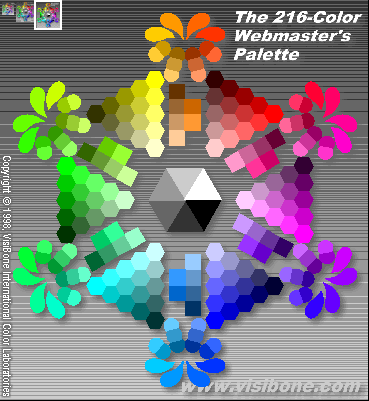
\includegraphics[width=.5\linewidth]{ColorMapNormal.png}
  \caption{As seen by a normal person}
  \label{fig:sub1}
\end{subfigure}%
\begin{subfigure}{.5\textwidth}
  \centering
  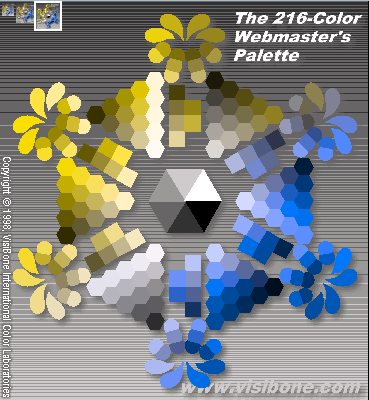
\includegraphics[width=.5\linewidth]{ColorMapCVD.png}
  \caption{As seen by CVD person (Protanopia)}
  \label{fig:sub2}
\end{subfigure}
\caption{Color Palette}
\label{fig:test}
\end{figure}

As we can observe, a CVD person can only see a subset of all possible colors. In other words, an entire set of colors(Fig 3.4(a)) is mapped to only a few different colors(Fig 3.4(b)). It is very probable that if two random colors are put into a single web page, they map to two colors that have very little differentiability between them. If they are used in background and text formatting, a color blind person won't be able to read the text, which might be a crucial aspect from a website designers point of view. To resolve this, we need a particular set of colors, which when used together, map to colors having significant differentiability for a CVD user.


Lets say there are two colors in a web page \textit{C1} and \textit{C2} as seen by a normal person. They will be seen as \textit{C1'} and \textit{C2'} by a CVD user. \textit{C1'} and \textit{C2'} should be differentiable enough for a CVD person to read the content on the web page. Idea is to replace \textit{C1} and \textit{C2} with \textit{D1} and \textit{D2} such that \textit{D1'} and \textit{D2'}, as seen by a CVD user, are differentiable enough.





\subsubsection{Limitations of this approach}
\label{Limitatios}

\begin{itemize}
\item{We will have to manually generate a finite number of sets from the palette available at [5], so that we can choose a particular set while recoloring.} 
\item{Still, there can be a case in which none of the colors in \textit{ColorHex} belongs to any of the sets, which restricts the scope of this approach.}
\item{This approach leads to bad \textit{perceptual naturalness}, as the complete set of original CSS colors will be replaced with a newer one.}
\end{itemize}


\subsection{SPRWeb}
\label{SPRWeb}

SPRweb[] by David et. al. is a tool that recolors websites to preserve subjective responses and improve color differentiability – thus enabling users with CVD to have similar on-line experiences. To recolor web pages, it uses a mapping available in DTEP(Dichromacy Trichromacy Equivalence Plane) set.


To find the DTEP set previous researches, have used findings from unilateral dichromats (individuals who are dichromatic in one eye, but are trichromatic in the other) to identify the set of colors that are perceived identically in dichromatic color vision and typical color vision. 

DTEP set contains all the colors which are perceived same as by a normal person and a CVD person. It also lists all the colors which are perceived by a CVD person. 

The key difference in our initial approach and that of SPRweb is the availability of a bigger set of colors and the inclusion of optimization of cost corresponding to \textit{perceptual naturalness}, \textit{perceptual differentiability}, \textit{subjective naturalness} and \textit{subjective differentiability.}

We developed following algorithm implementing approach mentioned in SPRWeb to compare its performance with our final algorithm. 


\makeatletter
\def\BState{\State\hskip-\ALG@thistlm}
\makeatother

\begin{algorithm}[!htb]
\caption{SPRWeb}\label{SPRWeb}
\begin{algorithmic}[1]
\Procedure{SPRWeb(CSSFile)}{}
\State ${ColorsHex,ColorMap} \gets \textit{CSSParser(CSSFile)}$
\State $ColorsOrig \gets HexToCIELab(ColorsHex)$
\State $DTEPSampled \gets UniformSample(DTEP,900)$ \Comment{gets 900 uniform samples from DTEP}
\State $ColorsRep \gets RAND(DTEPSampled,ColorsOrig.length)$ \Comment{Initializing Replaced color set with random colors from DTEPSampled}
\State $FirstOuput \gets FirstPass(ColorsOrig,ColorsRep,DTEPSampled)$
\For{$i \gets 1 \textrm{ to } FirstOuput.length$}
	\For{$j \gets 1\textrm{ to } DTEP$}
		\If{$distance(FirstOuput[i],DTEP[j]) < 5$} \Comment {Looks for all the points at 5 Lab units }
			\State $DTEPFiltered[i].append(DTEP[j])$
		\EndIf
	\EndFor
\EndFor
\State $FinalOutput\gets SecondPass(ColorsOrig,FirstOuput,DTEPFiltered)$
\State $ColorsHex \gets CIELabToHex(FinalOutput)$
\State $NewCSSFile \gets ReplaceColors(CSSFile, ColorsHex, ColorMap)$
\State \textbf{return} $NewCSSFile$
\EndProcedure
\algstore{myalg}

\end{algorithmic}
\end{algorithm}

\begin{algorithm}[!htb]
\caption{SPRWeb:continue}\label{SPRWeb:continue}
\begin{algorithmic}[1]
\algrestore{myalg}
\Procedure{FirstPass(ColorsOrig,ColorsRep,DTEPSampled)}{}
\State $cost \gets CalculateCost(ColorsOrig,ColorsRep)$
\State $ColorRep1 \gets ColorsRep$  \Comment{Initializing a variable to check optimization}
\While {$\textbf{true}$}
	\For{$i \gets 1 \textrm{ to } ColorsRep.length$}
		\For{$j \gets 1\textrm{ to } DTEPSampled$}
			\State $Value \gets ColorsRep[i]$
			\State $ColorsRep[i] \gets DTEPSampled[j]$ \Comment{trying a new color from DTEPSampled}
			\State $NewCost \gets CalculateCost(ColorsOrig,ColorsRep)$  \Comment{Calculating new cost after the change}
	        \If{$NewCost > cost$} 
	        		\State $ColorsRep[i] \gets Value$ \Comment{increased cost, Rejecting the color}
	        	\EndIf
	        \EndFor
	      \EndFor
	\State $ColorsRep2 \gets ColorsRep1$
	\State $ColorsRep1 \gets ColorRep$
	\If{$ColorsRep1 == ColorRep2$}
		\State $\textbf{break}$
	\EndIf
\EndWhile
\State $\textbf{return}  ColorRep1$
\EndProcedure
\Procedure{CSSParser(CSSFile)}{}
\State \textit{Defined in Algorithm 1}
\EndProcedure
\Procedure{ReplaceColors(CSSFile, ColorsHex, ColorMap)}{}
\State \textit{Defined in Algorithm 1}
\EndProcedure
\algstore{myalg}
\end{algorithmic}
\end{algorithm}

\begin{algorithm}[!htb]
\caption{SPRWeb:continue}\label{SPRWeb:continue2}
\begin{algorithmic}[1]
\algrestore{myalg}
\Procedure{SecondPass(ColorsOrig,ColorsRep,DTEPFiltered)}{}
\State $cost \gets CalculateCost(ColorsOrig,ColorsRep)$
\State $ColorRep1 \gets ColorsRep$  \Comment{Initializing a variable to check optimization}
\While {$\textbf{true}$}
	\For{$i \gets 1 \textrm{ to } ColorsRep.length$}
		\For{$j \gets 1\textrm{ to } DTEPFiltered[i]$}
			\State $Value \gets ColorsRep[i]$
			\State $ColorsRep[i] \gets DTEPFiltered[i][j]$ \Comment{trying a new color from DTEPSampled}
			\State $NewCost \gets CalculateCost(ColorsOrig,ColorsRep)$  \Comment{Calculating new cost after the change}
	        \If{$NewCost > cost$} 
	        		\State $ColorsRep[i]\gets Value$ \Comment{increased cost, Rejecting the color}
	        	\EndIf
	        \EndFor
	      \EndFor
	\State $ColorsRep2 \gets ColorsRep1$
	\State $ColorsRep1 \gets ColorRep$
	\If{$ColorsRep1 == ColorRep2$}
		\State $\textbf{break}$
	\EndIf
\EndWhile
\State $\textbf{return}  ColorRep1$
\EndProcedure
\algstore{myalg}
\end{algorithmic}
\end{algorithm}

\begin{algorithm}[!htb]
\caption{SPRWeb:continue}\label{SPRWeb:continue3}
\begin{algorithmic}[1]
\algrestore{myalg}
\Procedure{CalculateCost(ColorsOrig,ColorsRep)}{}
\State $pn \gets PercepNaturalness(ColorsOrig,ColorsRep)$
\State $pd \gets PercepDifferentiability(ColorsOrig,ColorsRep)$
\State $spn \gets SubNaturalness(ColorsOrig,ColorsRep)$
\State $spd \gets SubDifferentiability(ColorsOrig,ColorsRep)$
\State $cost \gets pn + pd + spn + spd$
\State \textbf{return} $cost$
\EndProcedure

\Procedure{PercepNaturalness(ColorsOrig,ColorsRep)}{}
\State $pn \gets 0$
\For{$i \gets 1 \textrm{ to } ColorsOrig.length$}
	\State $pn \gets pn + distance(ColorsOrig[i],ColorsRep[i])$
\EndFor
\State $pn \gets pn/ColorsOrig.length$
\State \textbf{return} $pn$
\EndProcedure

\Procedure{PercepDifferentiability(ColorsOrig,ColorsRep)}{}
\State $pd \gets 0$
\For{$i \gets 1 \textrm{ to } ColorsOrig.length$}
	\For{$j \gets i+1 \textrm{ to } ColorsRep.length$}
		\State $pd \gets pd + abs(distance(ColorsOrig[i],ColorsOrig[j]) - distance(ColorsRep[i],ColorsRep[j]))$
	\EndFor
\EndFor
\State $pd \gets pd/((ColorsOrig.length)*(ColorsOrig.length-1))$
\State \textbf{return} $pd$
\EndProcedure
\algstore{myalg}
\end{algorithmic}
\end{algorithm}

\begin{algorithm}[!htb]
\caption{SPRWeb:continue}\label{SPRWeb:continue4}
\begin{algorithmic}[1]
\algrestore{myalg}
\Procedure{SubNaturalness(ColorsOrig,ColorsRep)}{}
\State \textbf{return} $PercepNaturalness(Sub(ColorsOrig),Sub(ColorsRep))$
\EndProcedure
\Procedure{SubDifferentiability(ColorsOrig,ColorsRep)}{}
\State \textbf{return} $PercepDifferentiability(Sub(ColorsOrig),Sub(ColorsRep))$
\EndProcedure
\Procedure{Sub(Color)}{}   \Comment{Transforms a color to the subjective space}
\State $L \gets Color[0]$
\State $a \gets Color[1]$
\State $b \gets Color[2]$
\If{$a == 90$}
	\State $H \gets 90$
\Else
	\State $H \gets tan^{-1}b/a$
\EndIf
\State $C \gets sqrt({a^{2}+b^{2}})$
\State $activity \gets -2.1 + 0.06*sqrt({(l-50)^{2}+(a-3)^{2}+((b-17)/1.4)^{2}})$
\State $temp\gets -0.5 + 0.02*C^{1.07}*cos(H-50)$
\State $weight\gets -1.8 + 0.04*(100-l) + 0.45*cos(H-100)$
\State \textbf{return} ($activity$,$temp$,$weight$)
\EndProcedure
\end{algorithmic}
\end{algorithm}


\subsection{Performance Improvement in SPRWeb} 
\label{Improvement in SPRWeb}



While implementing SPRWeb to do performance comparison, we came across some redundant calculations which were happening at every step. By storing the result of those calculations once and then reusing them gave us a significant performance improvement.

\begin{itemize}
\item {Improvement Naturalness cost calculation:} Procedure \textit{PercepNaturalness} in Algorithm 6 computes a summation and has a time complexity of \textbf{O(n)} where n is the number of colors parsed from CSS file. And \textit{PercepNaturalness} is called every time we make a change in our \textit{ColorRep} set during optimization.

Instead of computing whole summation every time, we can compute the summation only once and then make changes in that for further replacement (because at each step only one color is being replaced and we can just change the sum according to that rather than re-computing whole summation), thus reducing computations.

We can rewrite our \textit{PercepNaturalness} procedure as shown in Algorithm 8. As we can see that the \text{for} loop for summation will get executes only once. Thus the time complexity of one call to \textit{PercepNaturalness} has an average cost of \textbf{O(1)} instead of \textbf{O(n)}.

Some other changes such as passing the value of of the index where the colors is getting replaced and the value of color which is getting replaced will have to be passed as well to the \textit{CalculateCost} procedure. But they all can be done without any added complexity. 

\begin{algorithm}[!htb]
\caption{Improvements in SPRWeb}\label{Improvements Naturalness}
\begin{algorithmic}[1]
\Procedure{PercepNaturalness(ColorsOrig,ColorsRep,$k$,OldColor)}{} \Comment{k=index of replacement, OldColor = Color being replaced}
\If {$pn == InitialzedValue$}  \Comment{is true only once - during first computation of cost}
		\For{$i \gets 1 \textrm{ to } ColorsOrig.length$}
			\State $pn \gets pn + distance(ColorsOrig[i],ColorsRep[i])$
		\EndFor
	\State $pn \gets pn/ColorsOrig.length$
\Else
\State $pn \gets pn*ColorsOrig.length$
\State $pn  \gets pn - distance(ColorsOrig[k],OldColor) + distance(ColorsOrig[k],ColorRep[k])$ 
\EndIf
\State \textbf{return} $pn$
\EndProcedure
\end{algorithmic}
\end{algorithm}

\item {Improvement differentiability cost calculation:}  Procedure \textit{PercepDifferentiability} in Algorithm 6 computes a double summation and has a time complexity of \textbf{O($n^{2}$)} where $n$ is the number of colors parsed from CSS file. And \textit{PercepDifferentiability} is called every time we make a change in our \textit{ColorRep} set during optimization process.


Instead of computing the two summations every time, we can compute the inner summation only once and then make changes in that for further replacement (because at each step only one color is being replaced and we can just change the sum according to that change rather than re-computing the double summation), thus reducing computations.

We can rewrite our \textit{PercepDifferentiability} procedure as shown in Algorithm 9. As we can see that the inner \text{for} loop for summation will get executes only once. Thus the time complexity of one call to \textit{PercepNaturalness} has an average cost of
O(n).


\begin{algorithm}[!htb]
\caption{Improvements in SPRWeb}\label{Improvements differentiability}
\begin{algorithmic}[1]
\Procedure{PercepDifferentiability(ColorsOrig,ColorsRep,$k$,OldColor)}{} \Comment{k=index of replacement, OldColor = Color being replaced}
\If {$pd == InitialzedValue$}  \Comment{is true only once - during first computation of cost}
		\For{$i \gets 1 \textrm{ to } ColorsOrig.length$}
			\For{$j \gets i+1 \textrm{ to } ColorsRep.length$}
				\State $pd \gets pd + abs(distance(ColorsOrig[i],ColorsOrig[j]) - distance(ColorsRep[i],ColorsRep[j]))$
			\EndFor
		\EndFor
		\State $pd \gets pd/((ColorsOrig.length)*(ColorsOrig.length-1))$
\Else 
\State $pd \gets pd*((ColorsOrig.length)*(ColorsOrig.length-1))$
\For{$i \gets 1 \textrm{ to } ColorsOrig.length$}
	\State $pd  \gets pd - abs(distance(ColorsOrig[i],ColorsOrig[k]) - distance(ColorsRep[i],OldColor))$
	\State $pd  \gets pd + abs(distance(ColorsOrig[i],ColorsOrig[k]) - distance(ColorsRep[i],ColorRep[k]))$
\EndFor
\State $pd \gets pd/((ColorsOrig.length)*(ColorsOrig.length-1))$
\EndIf
\State \textbf{return} $pd$
\EndProcedure
\end{algorithmic}
\end{algorithm}


\end{itemize}

\section{FBRecolor}
\label{FBRecolor}
While browsing the content on-line, specially reading, color of the text and the background are of key significance. Contrast between those two colors is one of the several important factors among other factors as mentioned in Definitions sections. SPRWeb tries to optimize the cost corresponding to perceptual naturalness, perceptual differentiability, subjective naturalness and subjective differentiability for the entire parsed set of colors. But at the very instant when user is reading a particular element of a web page, he/she may not be concerned about the other elements of the page. Therefore, we can optimize the cost corresponding to various factors for a particular element of the web page first and then repeat the same process for all the remaining elements. 


\subsection{Key idea} % (fold)
\label{Key idea}

% subsection subsection_name (end)
The idea is that while optimizing the various factors for a particular element rather than the whole web page, we will have more color options to choose from and thus the possibility of doing quantitatively better.


We divide a web page in elements based on the foreground-background color combination. For example, if a web page has two division elements, each having one color for background and one for the foreground text color, then the web page has two elements to be processed. Each element having one foreground-background(fg-bg) color pair. We define, a color pair as a combination of foreground and background for a particular element on a page.

Initial step of our algorithm parses out such fg-bg color pairs. Such fg-bg color pairs can be extracted by analysis of HTML Document Object Model(DOM) structure and CSS files. One of the possible implementations is shown later in the section. Once we have all the the color pairs parsed out, we perform our algorithm on each of the color pair. Pseudo code of the algorithm is given in Algorithm 10. A textual description is given in next section.

\subsection{Implementation} % (fold)
\label{Implementation}

% subsection su (end)

\textbf{FBRecolor} defines our tool. The input is the CSS file corresponding to the web page and the Document Object Model(DOM) of the web page. Output is a CSS file which is recolored using our tool. \textbf{FBRecolor} calls \textbf{NewCSSParser} whose input is also a CSS file and the DOM structure. The output is the pairs of foreground-background colors present in the CSS file. Procedure like \textbf{NewCSSParser} can be implemented by analyzing the DOM model and the CSS file both. 


In the CSS file, we can read the contents as a string and use regular expressions to parse the IDs and classes which it has and their corresponding colors in block.A mapping can be maintained which has IDs and .class as keys and a list as value. List contains the color properties(foreground and background) in that ID or class.

  
To analyze the DOM structure of HTML web page, we can use tools such as BeautifulSoup. The Default pair is foreground and background colors of the body tag. We can take a default value if they are not defined. Using such modules, we can traverse the DOM tree and check the class or ID which they are using. If no class or IDs or font color attributes are present that means they simply inherit the color of the parent and no new color is added to the system. But if there is some ID or class or color or font color defined, we retrieve its color property from dictionary maintained and report a new pair. Pairs are stored in separate lists like foreground color in one list and background color in other list. 


After we obtain a \textbf{Foreground} and \textbf{Background} color list, we pass one pair at once to procedure \textbf{FindRecolor}. \textbf{FindRecolor} returns the recolored pair corresponding to the input color. It optimizes the naturalness and differentiability among pairs. The three major steps which are present in \textbf{FindRecolor} can be explained as follows:

\begin{itemize}

\item {\textbf{Preserving naturalness:} } In the first step, we find a replacement $fg^{\prime}$ of a color $fg$ from a pair fg-bg in DTEP space. The replacement is such that the distance between $fg$ and $fg^{\prime}$ is as minimum as possible. This optimization maintains one of the perceptual naturalness as defined in SPRWeb[]. This ensures that the replacement color is as close to the original color as possible and there is no dramatic shift in replacement colors from original colors.

\item{\textbf{Preserving differentiability:} } In the second step, we draw a shell around $fg^{\prime}$ with internal radius as $d-e$ and outer radius as $d+e$, to obtain a possible set of colors for choosing a replacement $bg^{\prime}$ for $bg$. $d$ is the distance between original fg-bg color and $e$ is the factor introduced to ensure that we reach a solution. This step optimizes the perceptual differentiability property. This perceptual differentiability is different from what defined in SPRWeb. According to this property we try to maintain the contrast as it was present in original pair.

\item{\textbf{Preserving naturalness:} } In the third step, we choose a replacement $bg^{\prime}$ for $bg$ in possible set $bg$ such that the distance between $bg$ and $bg^{\prime}$ is minimum, again maintaining the perceptual naturalness property. 

\end{itemize}

After we obtain the list of replacements for \textbf{Foreground} and \textbf{Background}, we need a list of replacement colors of size equal to original colors present CSS file. Such a list is needed to replace colors back in original CSS and also to make sure that if a color is present in both background and foreground of different elements, then no conflict should arise. To achieve this, we first search for a color, present in original color list, in Foreground and Background color list. If the same color is present both in Foreground and Background then that means we have two candidate replacements for the same color. We choose a replacment for both the colors such that we get minimum cost of naturalness and differentiability in the pairs that contain those two colors. 

If a color is present only in Foreground and Background then we just put replacement of Foreground or Background in the replacement color list. 

After obtaining the replacement color list, we rewrite the CSS files reflecting new colors. 

\begin{algorithm}[!htb]
\caption{FBRecolor}\label{Our Approach}
\begin{algorithmic}[1]
\Procedure{FBRecolor(CSSFile,DOM)}{}
\State ${Foreground,Background,ColorMap} \gets \textit{NewCSSParser(CSSFile,DOM)}$
\State $ColorsOrig \gets HexToCIELab(Foreground \textbf{U} Background)$
\For{$j \gets 1\textrm{ to } Foreground.length$}
	\State $RecoloredForeground[i], RecoloredBackground[i] \gets FindRecolor(HexToCIELAB(Foreground[i]),HexToCIELAB(Background[i]))$
\EndFor
\For{$j \gets 1\textrm{ to } ColorsOrig.length$}
	\If{$Foreground.count(ColorsOrig[i])!= 0$}
	 \State $FIndex \gets Foreground.index(ColorsOrig[i])$
		\If {$Background.count(ColorsOrig[i])!=0$}
			\State $BIndex \gets Background.index(ColorsOrig[i])$
	\State $i \gets x such min{dist(RecoloredForeground[x],RecoloredBackground[x])-dist(Foreground[x],Background[x])+ dist(RecoloredForeground[x],Foreground[x]),x \in{FIndex,BIndex} }$
			\State $ColorRecolor[i] \gets ColorsOrig[i]$
		\Else
		\State $ColorRecolor[i] \gets RecoloredForeground[FIndex]$
		\EndIf	
	\EndIf
	\State $ColorRecolor[i] \gets RecoloredBackground[Background.index(ColorsOrig[j])]$
\EndFor
\State $ColorsHex \gets CIELabToHex(ColorRecolor)$
\State $NewCSSFile \gets ReplaceColors(CSSFile, ColorsHex, ColorMap)$
\State \textbf{return} $NewCSSFile$
\EndProcedure
\algstore{myalg}
\end{algorithmic}
\end{algorithm}


\begin{algorithm}[!htb]
\caption{FBRecolor:continue}\label{FBRecolor:continue}
\begin{algorithmic}[1]
\algrestore{myalg}
\Procedure{FindRecolor(fg,bg)}{}
\State $minDist = MAXINF$
\For{$j \gets 1\textrm{ to } DTEP$}
	\If{$distance(bg,j) < minDist$}
		\State $minDist = distance(bg,DTEP[j])$
	\EndIf
\EndFor
\For{$j \gets 1\textrm{ to } DTEP$}
	\If{$distance(bg,j) < minDist+0.5$}
		\State $minDistCircle .append(distance(bg,DTEP[j]))$
	\EndIf
\EndFor
\State $initialDifferentiability \gets distance(fg,bg)$
\State $a \gets 1$
\State $possibleSet \gets 0$
\While{$possibleSet.length <=0 $}
	\For{$j \gets 1\textrm{ to } DTEP$}
		\If {$(distance(minDistCircle[0],DTEP[j]) > initialDiffrentiablity - a*0.1  and distance(minDistCircle[0],DTEP[j]) < initialDiffrentiablity + a*0.1):$}
			\State $possibeSet.append(DTEP[j])$
		\EndIf
		\State $a = a*2$
	\EndFor
\EndWhile
\State $minDist \gets MAXINF$
\For{$j \gets 1\textrm{ to } possibleSet$}
	\If{$distance(fg,j) < minDist+0.5$}
		\State $minDist = distance(fg,possibleSet[j])$
		\State $replacementFg = possibleSet[j]$
	\EndIf
\EndFor
\State $\textbf{return} replacementFg,minDistCircle[0]$
\EndProcedure
\end{algorithmic}
\end{algorithm}



\section{Maintaining minimum contrast} % (fold)
\label{Maintaining minimum contrast}
Contrast is one of the major factors which is important in making a web page readable. In all the techniques discussed, measures are taken to ensure that the original colors and the contrast among them are preserved as much as possible. But there can be a case in which a color pair of replaced foreground and background exist which doesn't meeting the contrast criteria for reading.


\begin{figure}[!htb]
\centering
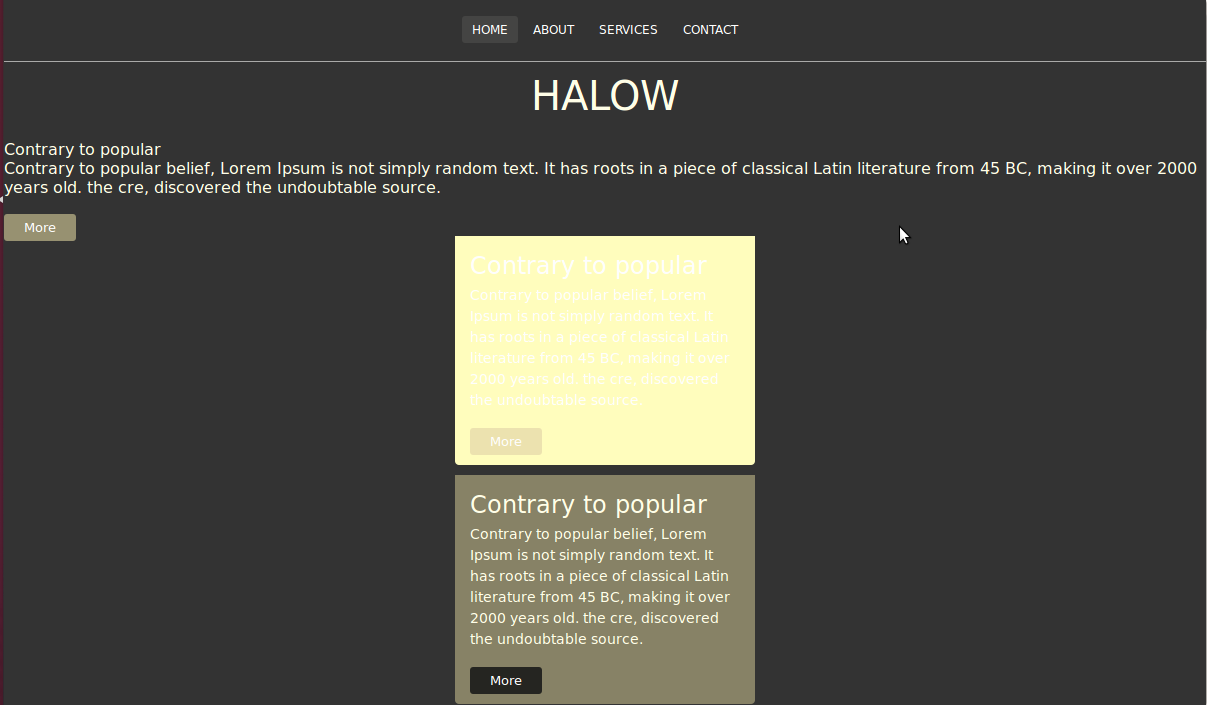
\includegraphics[width=.5\linewidth]{recolor.png}
\caption{Recoloring leading to bad contrast}
\label{fig:sub1}
\end{figure} 

To resolve such conflicts, we can follow the W3C guidelines of contrast threshold as provided in WCAG 2.0. 

\subsection{W3C guidelines} % (fold)
\label{W3C guidelines}

\begin{itemize}
\item{}this technique is needed to make sure that users can read text that is presented over a background. 

\item{}If the background is a solid color (or all black or all white) then the relative luminance of the text can be maintained by making sure that each of the text letters have 4.5:1 contrast ratio (CR) with the background.

\item{}If the background or the letters vary in relative luminance (or are patterned) then the background around the letters can be chosen or shaded so that the letters maintain a 4.5:1 contrast ratio with the background behind them even if they do not have that contrast ratio with the entire background.

\item{}For example, if a letter is lighter at the top than it is a the bottom, it may be difficult to maintain the contrast ratio between the letter and the background over the full letter. In this case, the designer might darken the background behind the letter, or add a thin black outline (at least one pixel wide) around the letter in order to keep the contrast ratio between the letter and the background above 4.5:1.

\item{}The contrast ratio can sometimes be maintained by changing the relative luminance of the letters as the relative luminance of the background changes across the page.

\end{itemize}

The procedure to implement the method as suggested by W3C is follows:

\begin{itemize}
\item{\textbf{Measure the relative luminance:}} of foreground text using the formula:
\begin{figure}[!htb]
  \centering
\[ L = 0.2126 * R + 0.7152 * G + 0.0722 * B\]
  \begin{tabular}{@{}>{$}l<{$}l@{}}
    $R$ & if $R_{sRGB} <= 0.03928$ then $R = R_{sRGB}/12.92$ else $R = ((R_{sRGB} + 0.055)/1.055)^{2.4}$\\
    $G$ & if $G_{sRGB} <= 0.03928$ then $G = G_{sRGB}/12.92$ else $G = ((G_{sRGB} +0.055)/1.055)^{2.4}$\\
    $B$ & if $B_{sRGB} <= 0.03928$ then $B = B_{sRGB}/12.92$ else $B = ((B_{sRGB} +0.055)/1.055)^{2.4}$\\
  	R_{sRGB} & $R_{8bit}/255$\\
  	G_{sRGB} & $G_{8bit}/255$\\
	B_{sRGB} & $B_{8bit}/255$\\
  \end{tabular}
\end{figure}

\item{}Measure the relative luminance of the background pixels immediately next to the letter using same formula.
\item{}Calculate the contrast ratio using the following formula.
\begin{figure}[!htb]
  \centering
\[ contrast = (L1 + 0.05) / (L2 + 0.05)\]
  \begin{tabular}{@{}>{$}l<{$}l@{}}
    $L1$ & Relative luminance of the lighter of the foreground or background colors\\
    $L2$ & Relative luminance of the darker of the foreground or background colors.\\
  \end{tabular}
\end{figure}
\item{}Check that the contrast ratio is equal to or greater than 4.5:1
\end{itemize}




\subsection{Including W3C guidelines in our approach} % (fold)
\label{Including W3C guidelines}

To include W3C guidelines in our approach, we analyzed the luminance values of the colors present in DTEP space. Following is the plot which was obtained: X-axis is index of DTEP color. Y-axis is luminance value. The graph is oscillating in nature.
\begin{figure}[!htb]
\centering
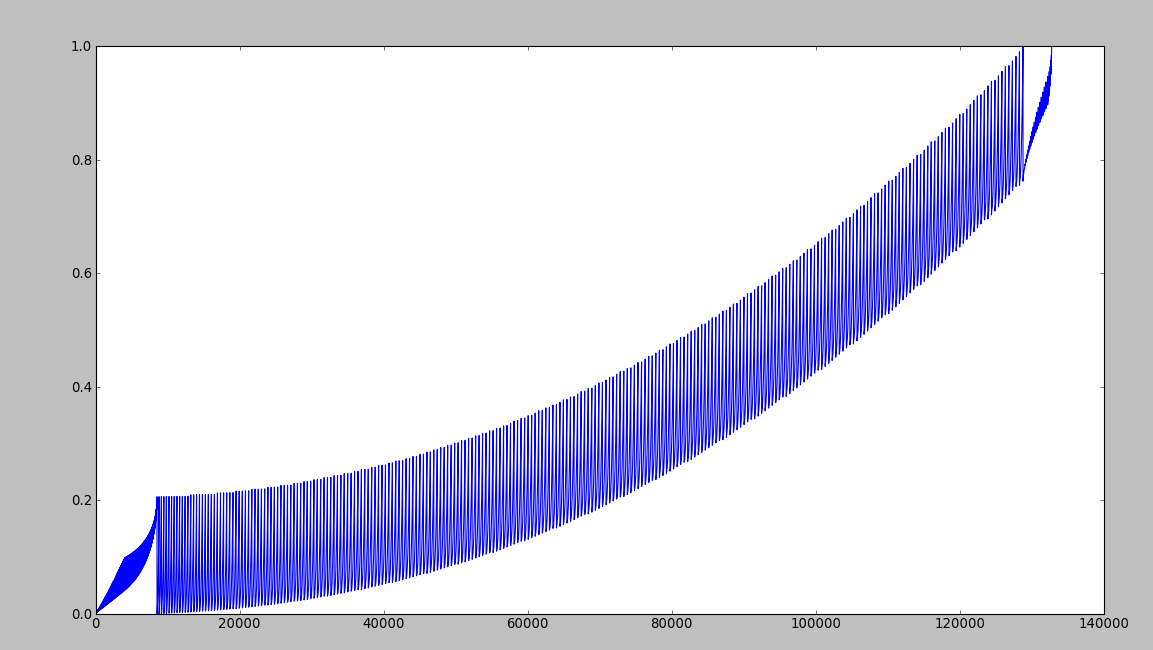
\includegraphics[width=\linewidth]{luminanceDTEP.png}
\caption{Luminance plot for DTEP}
\label{fig:LuminancePlot}
\end{figure} 

If we see the plot of contrast ratio of a color with the rest of DTEP colors, it would be as follows:
\begin{figure}[!htb]
\centering
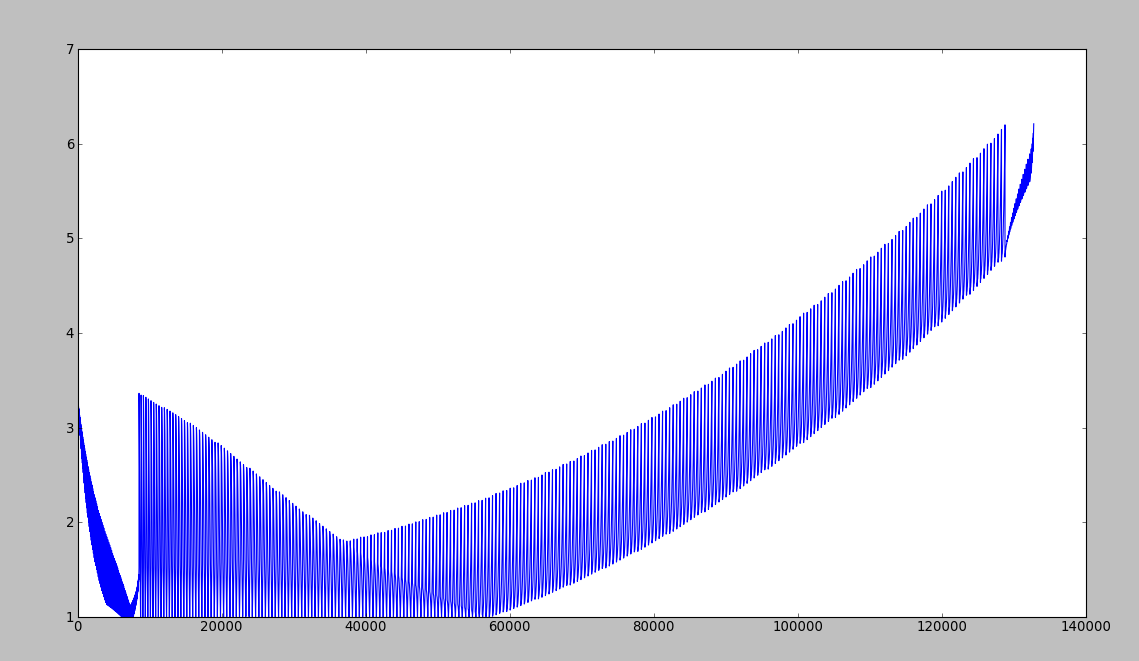
\includegraphics[width=\linewidth]{contrastDTEP.png}
\caption{contrast plot for DTEP}
\label{fig:ContrastPlot}
\end{figure}
If we observe we can see that the graph is particularly divided in two regions, one has a decreasing contrast ratio values followed by a unity point and then we have a region where contrast ratio is somewhat increasing. 


If we arrange the DTEP set according to the luminance values, we can obtain a graph like in Fig 3.8:
\begin{figure}[!htb]
\centering
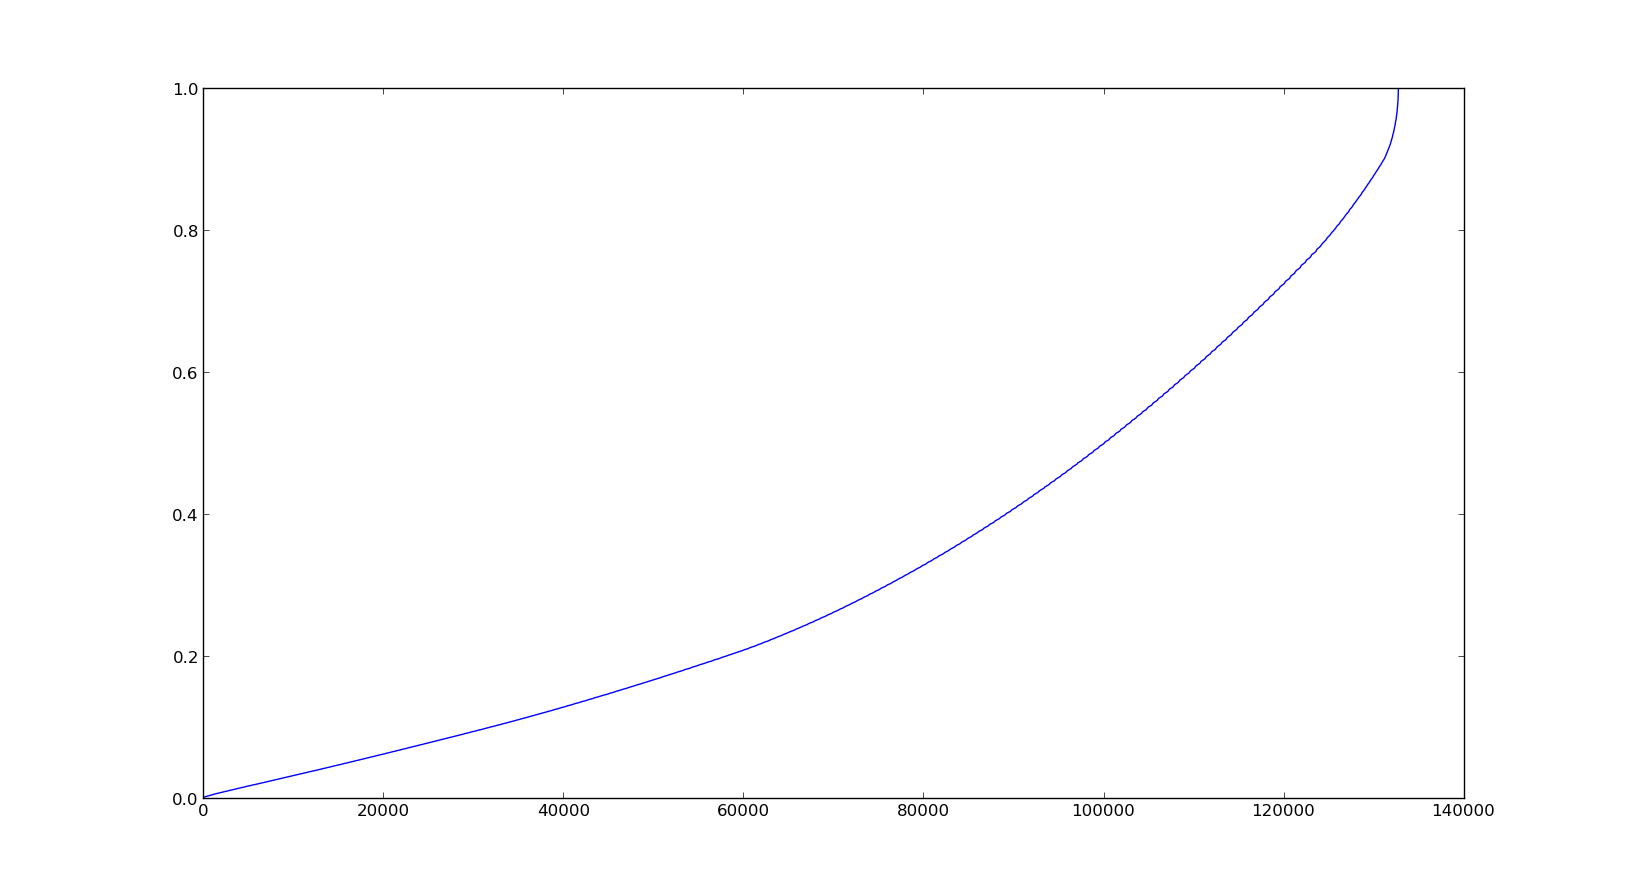
\includegraphics[width=\linewidth]{SortedLuminanceDTEP.png}
\caption{SortedLuminancePlot}
\label{fig:LuminanceSortedPlot}
\end{figure}



And using this same sorted DTEP set, we can obtain the contrast ratio graph of one of the colors, lets call A, and the rest of the DTEP members as shown in Fig 3.9.
\begin{figure}[!htb]
\centering
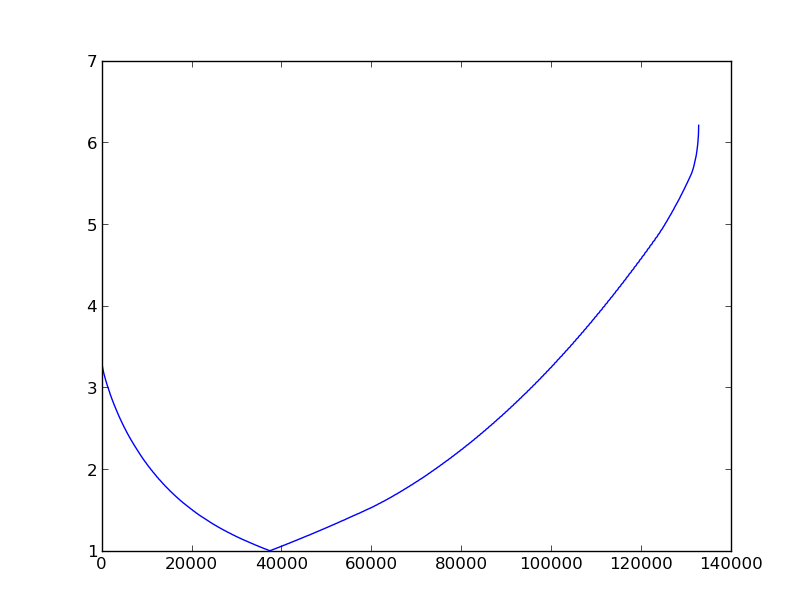
\includegraphics[width=\linewidth]{SortedContrast.png}
\caption{Sorted contrast plot}
\label{fig:SortedContrastPlot}
\end{figure}

As we can observe in Fig 3.9, value of the contrast ratio starts from a value, lets call it a starting point and then plunges to $0$. Lets call it a unity point. This unity point is essentially the index of occurrence of color A in DTEP set. After that, the contrast ratio increases and reaches its maximum value, lets call it a ending point.

Following observations can be made about starting point, unity point and ending point:
\begin{itemize}
\item{\textbf{Starting point can have a contrast value of [0,21])}} : As per the arrangement in DTEP set (increasing order of luminance), it is evident that maximum value of contrast ratio can occur at starting point when it is paired up with the last value of DTEP. 
\item {\textbf{Contrast ratio strictly declines from starting point till unity point}} : At unity point, the color is paired up with itself thus giving a contrast ratio of 1. If we move slightly to the left of unity point, we will see colors which have less luminance value as compared to the color A under consideration. And since the colors to the left have a luminance value less than that of A, their luminance value will be in the denominator of the CR formula. And as we move backwards towards the starting point, the denominator will keep on decreasing (due to the sorted luminance order in DTEP set), increasing the net CR value. 
\item{\textbf{Contrast ratio strictly increases from unity point till ending point}} : If we move slightly rightwards towards the ending point, the value of luminance in colors would increase. In the CR formula, luminance value of color on the right would be on top and that of color A, under consideration, would be in denominator. As we move right, numerator would increase, thus increasing net CR value. 
\end{itemize}



To make sure that the colors we choose satisfy the minimum contrast threshold criteria, we draw a vertical line $Y=4.5$ in Fig 3.9. The possible plots that can be obtained after that are shown in Fig. 3.10, 3.11 and 3.12:

\begin{figure}[!htb]
\centering
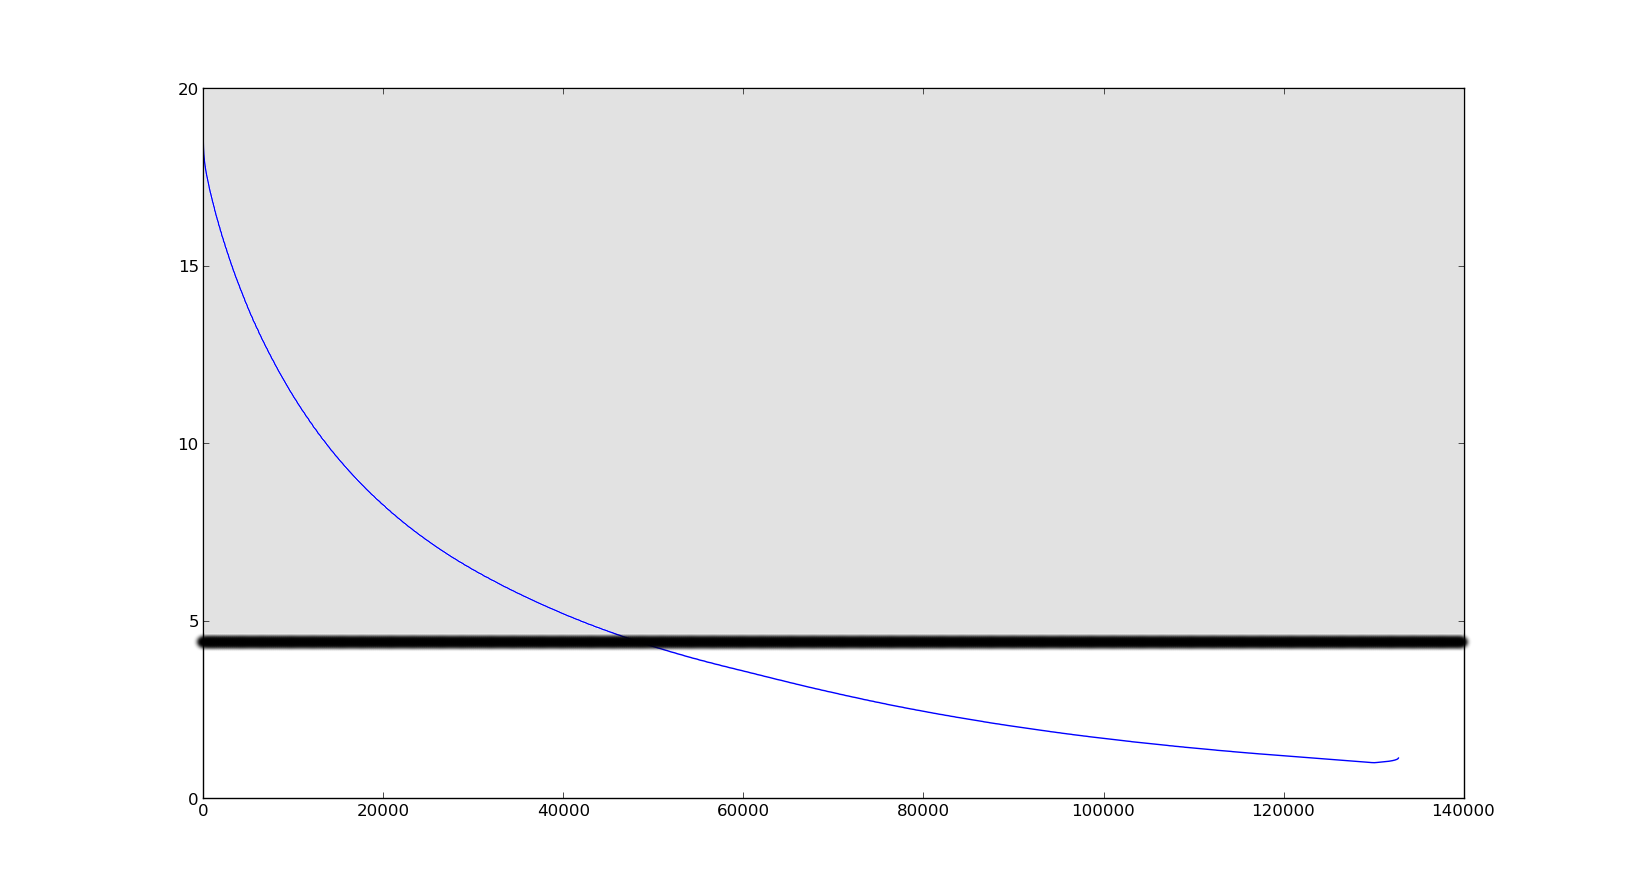
\includegraphics[width=\linewidth]{CR1.png}
\caption{Only starting point included}
\label{fig:sub1}
\end{figure}

\begin{figure}[!htb]
\centering
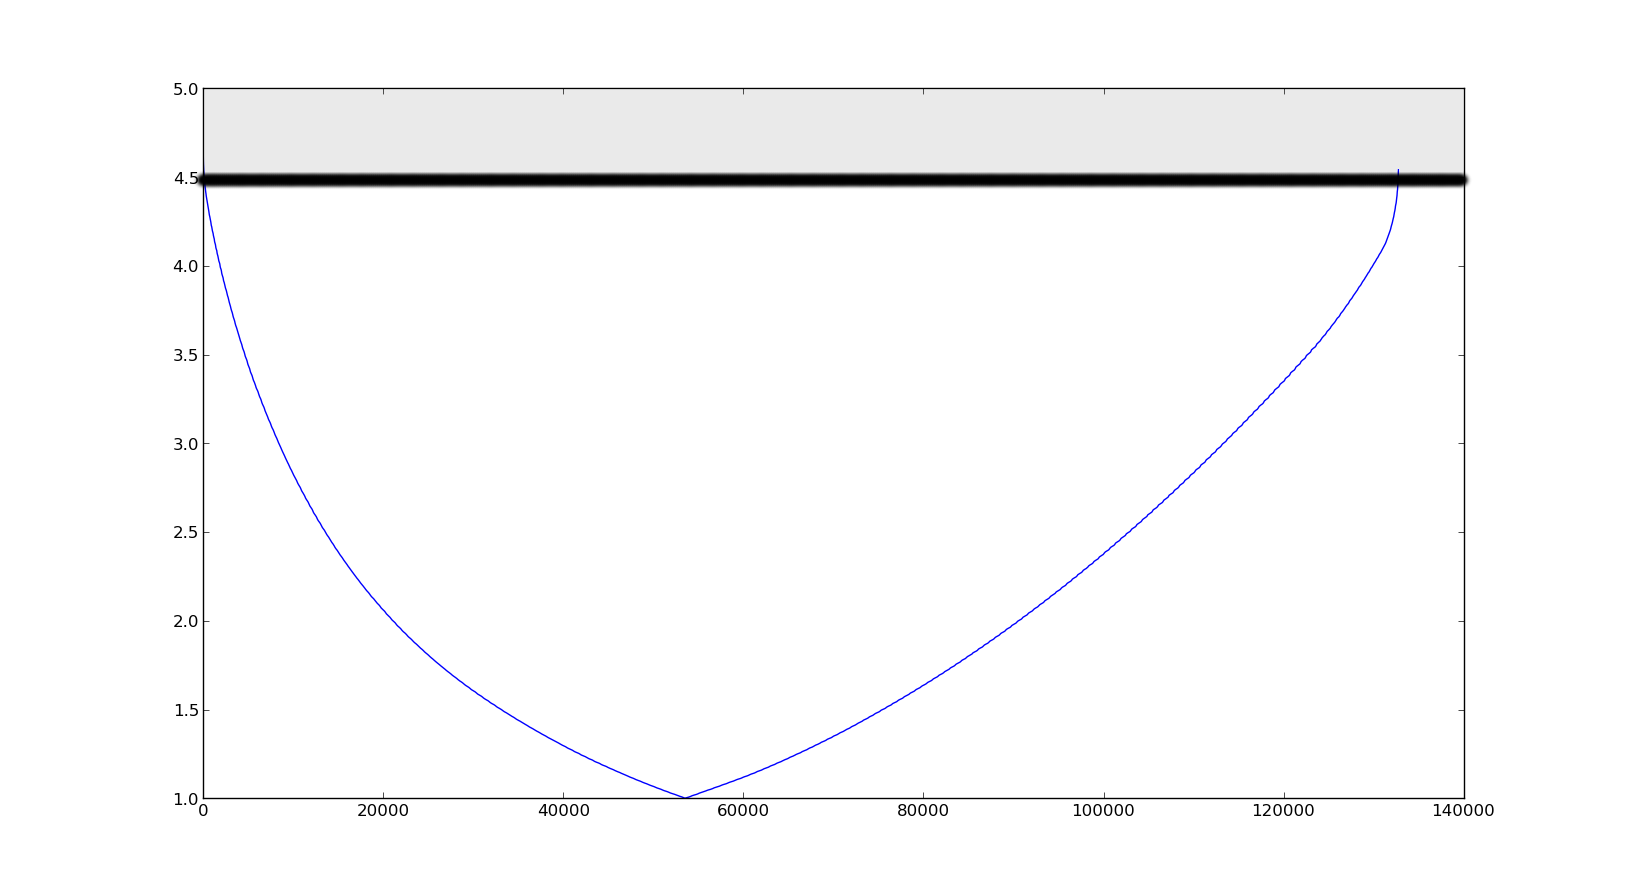
\includegraphics[width=\linewidth]{CR2.png}
\caption{Both starting and ending points included}
\label{fig:sub2}
\end{figure}

\begin{figure}[!htb]
\centering
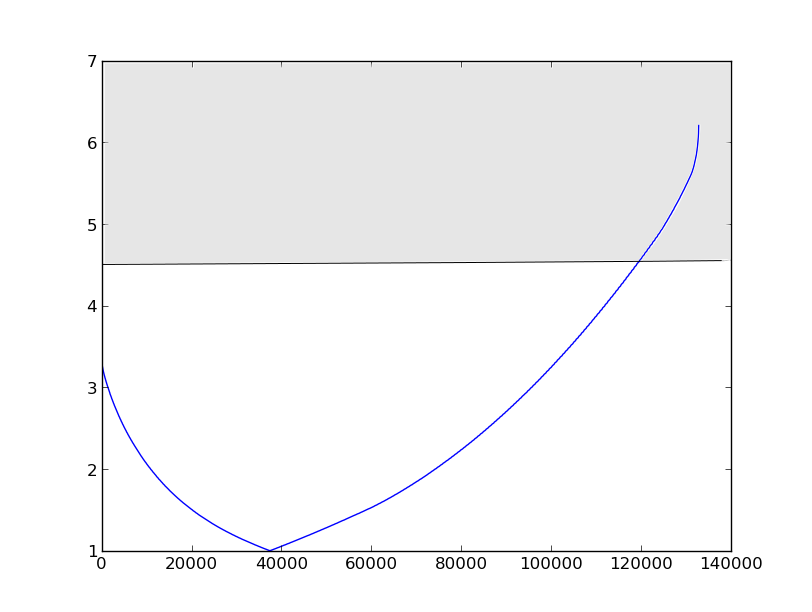
\includegraphics[width=\linewidth]{CR3.png}
\caption{Only ending point included}
\label{fig:sub3}
\end{figure}


The gray area in Fig 3.10,3.11 and 3.12 show the region from where we can take the colors such that the W3C guideline of minimum threshold is met.

\subsection{Implementation}
\label{Implementation}

Since we are aiming to make sure that the recolored web pages have color pairs such that the contrast ratio between them meets the 4.5:1 contrast threshold criteria, we need to restrict our possible color search space from DTEP set to a shorter set. Length and the properties of the possible set depends on the color being considered. As shown in Fig 3.10, 3.11, 3.12, the number of possibilities and their location depends on the color. A general approach to include this new criteria in recoloring of a pair, lets say fg-bg, would be to first find a replacement $fg^{\prime}$ for fg using the \textbf{FindRecolor} procedure in algorithm 11. And then obtain a curve like shown in Fig 3.10,11 and 12. Followed by finding the points which lie in the gray region in DTEP set and putting them in new \textit{DTEPReduced} set. And then finally searching a possible replacement $bg^{\prime}$ in the \textit{DTEPReduced} search space using the same approach as mentioned in \textbf{FindRecolor} procedure in algorithm 11. But since there are many pairs possible in a web page, obtaining a curve at run time for each and every pair adds to computational complexity. 

To resolve the problem of having to calculate the curves and find a \textit{DTEPReduced} set corresponding to a color in color pair, we pre-compute a mapping of possible values. This mapping has each color as a key and \textit{DTEPReduced} as value. A color, lets say x, has a \textit{DTEPReduced} set such that all colors in \textit{DTEPReduced} set when paired with x, produce a contrast ratio of more than 4.5. Thus, if in a pair fg-bg, where replacement for fg is $fg^{\prime}$, if we choose a replacement for bg in \textit{DTEPReduced} set, then we would be sure that the recolored pair $fg^{\prime}$-$bg^{\prime}$ has a contrast ratio of more than 4.5.

The mapping can be obtained using the procedure in Algorithm 12.
\begin{algorithm}[!htb]
\caption{Find Mapping}\label{Find Mapping}
\begin{algorithmic}[1]
\Procedure{FindMapping()}{}
\For{$j \gets 1\textrm{ to } DTEP$}
	\State $DTEPLuminance[j] \gets luminance(DTEP[j])$
\EndFor
\State $DTEPSorted \gets [x for (y,x) in sorted(zip(DTEPLuminance,DTEP))]$ \Comment{Sorting DTEP based on DTEPLuminance}
\State $DTEPLuminance \gets Sorted(DTEPLuminance)$ \Comment{sorting the list}
\For{$j \gets 1\textrm{ to } DTEPSorted$}
	\If{$ContrastRatioFinder(DTEPSorted[j],DTEPSorted[0]) < 4.5$}  \Comment{Taking care of Fig. 3.12}
		\State $Constant \gets 4.5*(DTEPLuminance[j]+0.05) - 0.05$
		\If{$Constant > 1$}
			\State $index \gets -1$
			\State	$Mapping[DTEPSorted[j]] \gets [len(DTEPLuminance)-index-j-1,(-1,-1)]$
		\Else
		\State $index \gets findGe(DTEPLuminance[j+1:len(DTEPLuminance)],Constant)$
		\State	$Mapping[DTEPSorted[j]] \gets [len(DTEPLuminance)-index-j-1,(index+j+1,len(DTEPLuminance))]$
		\EndIf
	\Else 		\Comment{Taking care of Fig 3.10 and Fig 3.11}											
	\State $Constant \gets (DTEPLuminance[j]+0.05)/4.5 - 0.05$
	\State	$index1 \gets findGe(DTEPLuminance[0:j],Constant)$
	\State $Constant \gets 4.5*(DTEPLuminance[j]+0.05) - 0.05$
	\EndIf
\algstore{myalg}
\end{algorithmic}
\end{algorithm}

\begin{algorithm}[!htb]
\caption{Find Mapping:continue}\label{Find Mapping}
\begin{algorithmic}[1]	
\algrestore{myalg}
	\If	{$Constant > 1$}
		\State $index2 \gets -1$
		\State $Mapping[DTEPSorted[j]] \gets [index1,(0,index1),(-1,-1)]$
	\Else		
	\State $index2 \gets findGe(DTEPLuminance[j+1:len(DTEPLuminance)],Constant)$
	\State $Mapping[DTEPSorted[j]] \gets [len(DTEPLuminance)-index2-j-1 + index1,(0,index1),(index2+j+1,len(DTEPLuminance))]$
	\EndIf
\EndFor
\textbf{return } $Mapping$
\EndProcedure
\Procedure{ContrastRatioFinder(color1, color2)}{}
\State Can be implemented easily using the lightness and contrast formula described above.
\EndProcedure
\Procedure{luminance(color)}{}
\State Can be implemented easily using the lightness formula described above. 
\EndProcedure
\Procedure{findGe(List, Constant)}{}
\Comment{Finds smallest item greater-than or equal to key.
    Raise ValueError if no such item exists.
    If multiple keys are equal, return the leftmost.
    }
\State $i \gets bisect.bisect_left(List, Constant)$
\If{$i == len(List)$}
    \State raise ValueError('No item found with Constant at or above)
\EndIf
\State \textbf{return} $i$
\EndProcedure
\end{algorithmic}
\end{algorithm}

Using the mapping obtained from Algorithm 13, we can modify procedure \textbf{FindRecolor} in Algorithm 11 as shown in Algorithm 14. 

\begin{algorithm}[!htb]
\caption{FBRecolor:Modified}\label{Minimum contrast included}
\begin{algorithmic}[1]
\Procedure{FindRecolor(fg,bg)}{}
\State $minDist = MAXINF$
\For{$j \gets 1\textrm{ to } DTEP$}
	\If{$distance(bg,j) < minDist$}
		\State $minDist = distance(bg,DTEP[j])$
	\EndIf
\EndFor
\For{$j \gets 1\textrm{ to } DTEP$}
	\If{$distance(bg,j) < minDist+0.5$}
		\State $minDistCircle .append(distance(bg,DTEP[j]))$
	\EndIf
\EndFor
\State $initialDifferentiability \gets distance(fg,bg)$
\State $maxOptions \gets -1000$
\For{$j \gets 1\textrm{ to } minDistCircle$}
		\If{$mapping[j].length> maxOptions$} \Comment{Mapping imported from Algorithm 13} 
		\State	$maxOptions \gets mapping[j].length$
		\State	$MaxMinDist \gets j$
		\EndIf
\EndFor
\State $a \gets 1$
\State $possibleSet \gets 0$
\While{$possibleSet.length <=0 $}
	\For{$i \gets 1\textrm{ to } mapping[j]$}
		\If {$(distance(minDistCircle[0],mapping[j][i]) > initialDiffrentiablity - a*0.1  and distance(minDistCircle[0],mapping[j][i]) < initialDiffrentiablity + a*0.1):$}
			\State $possibeSet.append(mapping[j][i])$
		\EndIf
		\State $a = a*2$
	\EndFor
\EndWhile
\State $minDist \gets MAXINF$
\algstore{myalg}
\end{algorithmic}
\end{algorithm}

\begin{algorithm}[!htb]
\caption{FBRecolor:Modified}\label{Minimum contrast included}
\begin{algorithmic}[1]
\algrestore{myalg}
\For{$j \gets 1\textrm{ to } possibleSet$}
	\If{$distance(fg,j) < minDist+0.5$}
		\State $minDist = distance(fg,possibleSet[j])$
		\State $replacementFg = possibleSet[j]$
	\EndIf
\EndFor
\State $\textbf{return} replacementFg,minDistCircle[0]$
\EndProcedure
\end{algorithmic}
\end{algorithm}

Algorithm 14 describes a one possible heuristic to obtain a output color set using the mapping. The heuristic is such that when we recolor a pair lets say fg-bg, and we have many possible replacements for fg. Then out of those possible replacements of fg, we choose a a replacement such that the length of the list in \textit{mapping} is maximum. In other words, we choose a value for fg such that we have a large number of option for bg. This gives us a possibility of reaching to a better solution in terms of naturalness and differentiability, since we have many options available. This is one possible heuristic to reach to the solution, several others heuristics can also be implemented. 

